\documentclass{beamer}

\usepackage{amsmath}
\usepackage[style=alphabetic,url=true]{biblatex}
\usepackage{environ}
\usepackage{geometry}
\usepackage{graphicx}
\usepackage{amsmath}
\usepackage{amsfonts}
\usepackage{amssymb}
\usepackage{calrsfs}
\usepackage{listings}
\usepackage{tikz}
\usepackage[T2A]{fontenc}
\usepackage[utf8]{inputenc}
\usepackage[cache=false]{minted}

\graphicspath{ {./graphics/} }
\usetikzlibrary{shapes.arrows,chains}
\usecolortheme{beaver}
\setbeamertemplate{itemize item}[circle]
\setbeamertemplate{itemize subitem}{--}
\addtobeamertemplate{navigation symbols}{}{
  \usebeamerfont{footline}
  \usebeamercolor[fg]{footline}
  \hspace{1em}
  \insertframenumber/\inserttotalframenumber
}
\setminted[Lisp]{
  fontsize=\scriptsize
}
\BeforeBeginEnvironment{minted}{\medskip}
\AfterEndEnvironment{minted}{\medskip}



\title{
  Common Lisp and Introduction to Functional Programming \\
  Lecture 6: Functional Programming Basics
}
\author{Yuri Zhykin}
\date{Mar 17, 2021}

\begin{document}

\frame{\titlepage}

\begin{frame}[fragile]
  \frametitle{Functions in Mathematics 1/2}
  \begin{itemize}
  \item In mathematics, a \textbf{function} is a \textit{binary relation}
    between \textit{two sets} that associates to each element of the first set
    \textit{exactly one} element of the second set.
  \item \textit{Intentionally}, functions can be defined as combinations of
    \textit{primitive operations} and \textit{previously defined functions}:
    $$f(x) = 10^x$$
  \item \textit{Extensionally}, functions can be defined by listing function
    values that correspond to argument values:
    $$f(x)=
    \begin{cases}
      10, &x = 1,\\
      100, &x = 2,\\
      1000, &x = 3,\\
      ... &...
    \end{cases}
    $$
  \end{itemize}
\end{frame}

\begin{frame}[fragile]
  \frametitle{Functions in Mathematics 2/2}
  \begin{itemize}
  \item Mathematical functions are often called \textbf{maps}
    or\textbf{mappings} between sets.
  \item Mathematics distinguish the following components of a function
    definition: \textbf{domain}, \textbf{codomain}, \textbf{image} and
    \textbf{graph}.
    \begin{center}
      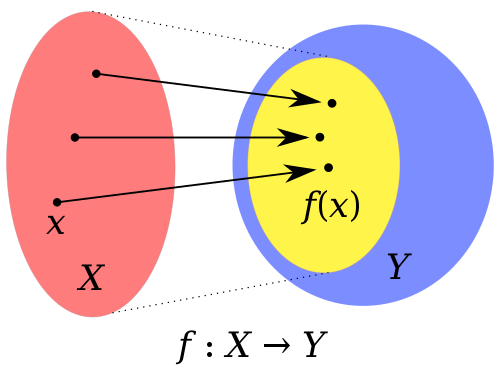
\includegraphics[width=0.3\textwidth]{xyg}
    \end{center}
  \item The output of a mathematical function depends only on the input, so one
    only needs the input value and the function definition itself denoted in
    some way in order to establish the corresponding output.
  \end{itemize}
\end{frame}

\begin{frame}[fragile]
  \frametitle{Functions in Programming}
  \begin{itemize}
  \item Commonly used term \textbf{function} in modern programming languages
    actually means \textbf{procedure}.
  \item \textbf{Procedures} are also known in some programming languages as
    \textbf{routines} or \textbf{subroutines}.
  \item \textbf{Procedural programming} is a programming paradigm based on the
    concept of the \textbf{procedure call}.
  \item \textbf{Procedure} is a group of instructions that do a clearly defined
    task and can be ``called'' multiple times - a very basic means of achieving
    \textbf{modularity} and \textbf{code reuse}.
  \item \textbf{Procedure} only vaguely resembles a mathematical function.
  \end{itemize}
\end{frame}

\begin{frame}[fragile]
  \frametitle{State}
  \begin{itemize}
  \item \textbf{What is the difference between a procedure and a mathematical
      function?}
  \item \textbf{State} of a program can be defined as the values of all
    variables (i.e. contents of all storage locations in memory) at any given
    point in time.
  \item By definition, the result of mathematical function depends solely on its
    arguments.
  \item Procedures (or ``functions'') in programming languages always depend on
    state of the program at the moment of procedure (or ``function'') call.
  \item In order to determine the result of the procedure call, we need to look
    at the whole program state, not just the procedure definition and arguments.
  \end{itemize}
\end{frame}

\begin{frame}[fragile]
  \frametitle{Side effects}
  \begin{itemize}
  \item \textbf{Let's make matters even more complicated!}
  \item Any useful program \textbf{modifies} the global state in order to produce
    useful results.
  \item Procedure's result can depend on parts of the state that is modified by
    any other procedures, including itself, so even sequential calls of the same
    procedure may produce different results.
  \item Modifications of variables or structures after they were defined are
    called \textbf{mutations}.
  \end{itemize}
\end{frame}

    
\begin{frame}[fragile]
  \frametitle{Practical Function Programming}
  \begin{itemize}
  \item \textbf{What if we wrote procedures in a way that does not depend on
      state?}
  \item We call all ``functions'' \textbf{procedures}.
  \item We agree to write \textbf{some} procedures in a way that does not
    \textbf{explicitly} depend on global state, and we call such procedures
    \textbf{functions} or \textbf{pure functions}.
  \item We call any modifications of the state \textbf{outside the scope} of a
    procedure \textbf{side effects}.
  \item We can treat procedures free of side effects as ``black boxes'' - as
    soon as we define and verify it, we no longer care about the internals.
  \item Our program is split into two parts - one that is free of side-effects,
    and the other that is responsible for all side effects.
  \end{itemize}
\end{frame}

\begin{frame}[fragile]
  \frametitle{Referential Transparency}
  \begin{itemize}
  \item An expression is called \textbf{referentially transparent} if it can be
    replaced with its corresponding value (and vice-versa) without changing the
    program's behavior.
\begin{minted}{Lisp}
  (defun the-answer ()
    (print "The answer is: 42.")
    42)

  ;; (+ 1 (the-answer))
  ;; (+ 1 42)
\end{minted}
  \item Expressions that consist of \textbf{pure function} calls are
    referentially transparent.
  \end{itemize}
\end{frame}

\begin{frame}[fragile]
  \frametitle{Recursion 1/2}
  \begin{itemize}
  \item N-th Fibonacci number function:
    $$Fib(n) = \begin{cases}
      0, &n = 0, \\
      1, &n = 1, \\
      Fib(n-1) + Fib(n-2), &\text{otherwise} \\
    \end{cases}$$    
  \item Imperative approach using loop:
\begin{minted}{Lisp}
  (defun fib (n)
    (let ((a 0) 
          (b 1))
      (loop :for i :below n :do
        (multiple-value-setq (a b) (values b (+ a b))))
      a))
\end{minted}
  \item Functional approach that follows mathematical definition:
\begin{minted}{Lisp}
  (defun fib (n)
    (if (or (= n 0) (= n 1))
        n
        (+ (fib (- n 1)) (fib (- n 2)))))
\end{minted}
  \end{itemize}
\end{frame}

\begin{frame}[fragile]
  \frametitle{Recursion 2/2}
  \begin{itemize}
  \item Using \textbf{recursion} as a general replacement for loops might be
    inefficient when following mathematical definitions, but most recursive
    functions can be written in a \textbf{tail-recursive} form.
  \item Function call requires more instructions than a loop iteration.
  \item \textbf{Tail recursion} refers to the recursive call being the last
    logic instruction in the recursive algorithm.
  \item Functional approach optimized with tail recursion:
\begin{minted}{Lisp}
  (defun fib (n)
    (labels ((%fib (%n a b)
               (if (= %n n)
                   a
                   (%fib (+ %n 1) b (+ a b)))))
      (%fib 0 0 1)))        
\end{minted}
  \item Some languages (e.g. Lisp) implement \textbf{TCO} (\textbf{tail call
      optimization}) that replaces a tail function call with a jump.
  \end{itemize}
\end{frame}

\begin{frame}
  \frametitle{The End}
  \begin{center}
    Thank you!
  \end{center}
\end{frame}

\end{document}

%%% Local Variables:
%%% mode: latex
%%% TeX-master: t
%%% TeX-command-extra-options: "-shell-escape"
%%% End:
